\documentclass[11pt]{beamer}
\usetheme{Warsaw}
\usepackage[utf8]{inputenc}
\usepackage[russian]{babel}
\usepackage[T2A]{fontenc}
\usepackage{amsmath}
\usepackage{amsfonts}
\usepackage{amssymb}
\usepackage{graphicx}
\author{Турганбаев Сатбек Амангельдыулы}
\title{Исследование метода восстановления волнового фронта по его наклонам\\ на основе вейвлетов Хаара}

%\setbeamercovered{transparent} 
%\setbeamertemplate{navigation symbols}{} 
%\logo{} 
\institute{Московский Государственный Университет имени М.В.Ломоносова \\
Факультет вычислительной математики и кибернетики \\
Кафедра математической физики \\
\vspace{\baselineskip}
Выпускная квалификационная работа бакалавра \\
\vspace{\baselineskip}
Научный руководитель: д.т.н., профессор Разгулин А.В.} 
\date{2018г.} 


\setbeamertemplate{navigation symbols}{}

\begin{document}

\begin{frame}
\titlepage
\end{frame}


\begin{frame}
\frametitle{Цель работы}

\begin{enumerate}
\item Реализовать вейвлет и вариационный методы восстановления волнового фронта
\item Исследовать их на различных представлениях наклонов волнового фронта
\end{enumerate}
\end{frame}

\begin{frame}
\frametitle{Постановка задачи}

Функция двух переменных $u(x,y)$ , ее производные имеют вид  $u_x(x,y)$, $u_y(x,y)$.



Введем сетку: 
$$
\omega_h = \{(x_i, y_j) \,:\, x_i = ih_1,\,y_j = jh_2,\, i = 0..N_1,\, j = 0..N_2;\; h_{1,2}N_{1,2} = 2\pi\}
$$
Матрицы $U,\, g_1,\, g_2$ являются дискретными представлениями функций $u(x,y) ,\, u_x(x,y) ,\, u_y(x,y)$ на сетке $\omega_h$.

\begin{block}{Задача восстановления  волнового фронта}
Задача восстановления волнового фронта состоит в приближенном восстановлении  матрицы матрицы $U$, по известным наклонам $g_1,\, g_2$.
\end{block}
\end{frame}

\begin{frame}
\frametitle{Различные представления }
\framesubtitle{наклонов волнового фронта}

\begin{enumerate}
\item Точные значения производных:\\$g_1 = u_x(x_i,y_j);\; g_2 = u_y(x_i,y_j)$
\item Первые разностные производные:\\
$g_1= \frac{u(x_i,y_j) - u(x_{i-1},y_j)}{h_1};\;g_2= \frac{u(x_i,y_j) - u(x_i,y_{j-1})}{h_2}$
\item Случай восстановления по средним локальным апертурам значений наклонов:\\$
g_1 = \frac{1}{h_1h_2} \sum \limits_{n=1}^{N_1 - 1} \sum \limits_{m=1}^{N_2 - 1} \int \limits _{\Delta_{nm}} u_\xi(\xi,\eta) d\xi d\eta\overset{\circ}{\varphi}_{nm}(x,y)
$\\
$
g_2 = \frac{1}{h_1h_2} \sum \limits_{n=1}^{N_1 - 1} \sum \limits_{m=1}^{N_2 - 1} \int \limits _{\Delta_{nm}} u_\eta(\xi,\eta) d\xi d\eta \overset{\circ}{\varphi}_{nm}(x,y)$
\end{enumerate}
\end{frame}

\begin{frame}
\frametitle{Вейвлет метод}


\begin{block}{}
Алгоритм метода состоит в получении разложения Хаара($_{HH}^{M-1}\Phi, _{HL}^{M-1}\Phi, _{LH}^{M-1}\Phi, _{HH}^{M-2}\Phi, \ldots $) волнового фронта по его локальным наклонам и применении к полученному разложению обратного преобразования Хаара
\end{block}

\begin{columns}
\begin{column}{0.5\textwidth}
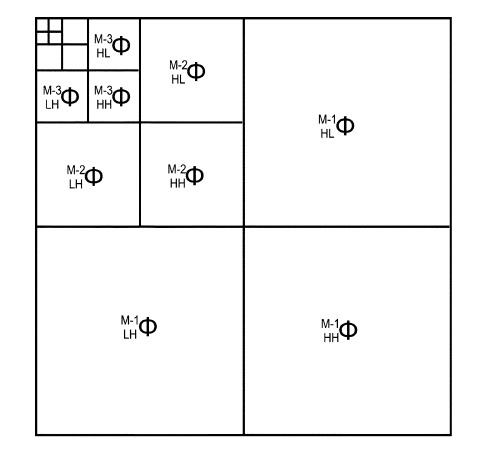
\includegraphics[width=\linewidth]{hwaf_decomp.png}
\end{column}

\begin{column}{0.5\textwidth}
$$g_1= \frac{u(x_i,y_j) - u(x_{i-1},y_j)}{h_1}$$
$$g_2= \frac{u(x_i,y_j) - u(x_i,y_{j-1})}{h_2}$$
\end{column}
\end{columns}
\end{frame}

\begin{frame}
\frametitle{Восстановление полиномов Цернике}
\framesubtitle{при различных представлениях наклонов}
Полином Цернике $R_3^3=\rho^3 $ 
\\в случае точных значений производных:
\begin{minipage}[h]{1\linewidth}
\center{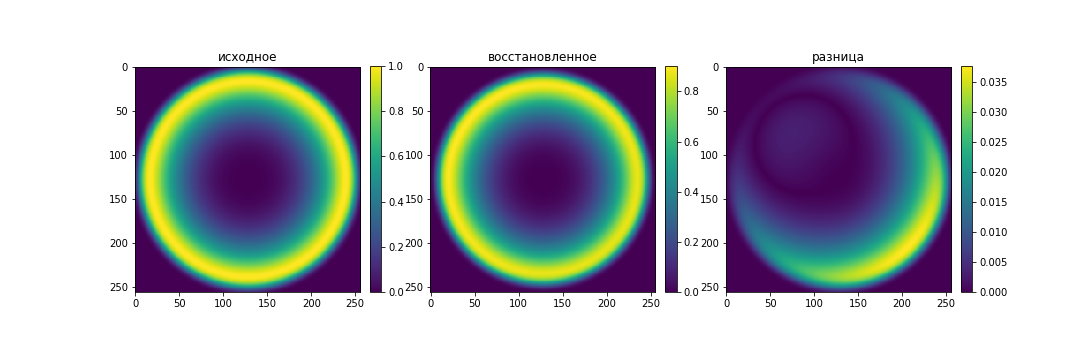
\includegraphics[width=0.8\linewidth]{R_3^3_variant1.png}}
\end{minipage}
\\в случае первых разностных производных:
\begin{minipage}[h]{1\linewidth}
\center{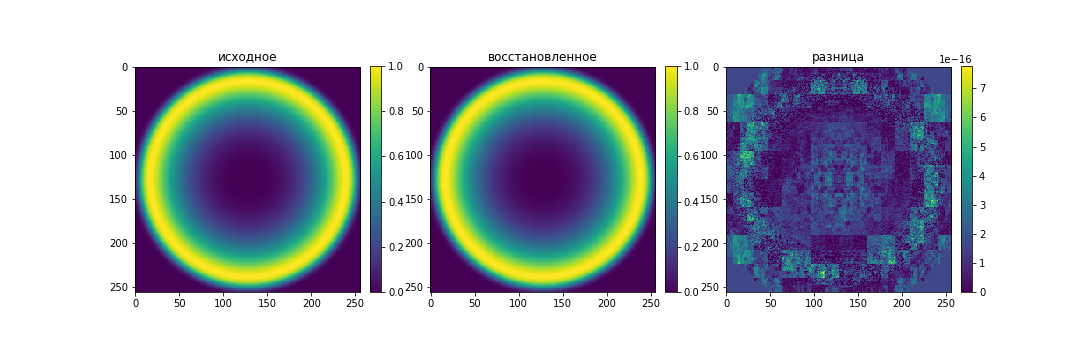
\includegraphics[width=0.8\linewidth]{R_3^3.png}}
\end{minipage}
\end{frame}

\begin{frame}
\frametitle{Вариационный метод}

\begin{block}{Минимизация функционала невязки}
$J(u) = \int \limits_0^{2\pi} \int \limits_0^{2\pi} ((u_x - g_1)^2 + (u_y-g_2)^2 + \alpha u^2 )dxdy \rightarrow min$
\end{block}
\begin{block}{Необходимое условие минимума функционала в форме интегрального тождества}
$(u_x, \phi_x) + (u_y,\phi_y) + \alpha(u, \phi) = (g_1, \phi_x) + (g_2, \phi_y)$\\$\forall\phi \in W_{2\pi}^{1}(\Omega),\;(\cdot\,,\cdot)$ - скалярное произведение в $L_2(\Omega)$
\end{block}
\end{frame}

\begin{frame}{Проекционно-разностная схема}
Определим на $\Omega$ систему финитных базисных функций $\{\phi_i(x)\} ,\, i \in [0,\,N-1]$.
$$
\phi_i(x) = 
 \begin{cases}
  \frac{x-x_{i-1}}{h} , x \in [x_{i-1},x_i] \\ 
   \frac{x_{i+1} - x}{h}, x \in [x_{i},x_{i+1}]   \\
   0 \notin [x_{i-1},x_{i+1}].
 \end{cases}\;
\phi_0(x) = 
 \begin{cases}
  \frac{x_1-x}{h} , x \in [x_{0},x_1] \\ 
   \frac{x - x_{N-1}}{h}, x \in [x_{N-1},x_{N}]   \\
   0 \in [x_{1},x_{N-1}].
 \end{cases}
$$
\begin{block}{}
Из необходимого условия минимума функционала $(u_x, \phi_x) + (u_y,\phi_y) + \alpha(u, \phi) = (g_1, \phi_x) + (g_2, \phi_y)$ получим проекционно-разностную схему
\end{block}
\begin{block}{Проекционно-разностная схема}
$$B_2 \Lambda_1 u + B_1 \Lambda_2 u + \alpha B_1 B_2 u + \gamma\Lambda_1\Lambda_2u = F(g_1,g_2)$$
$F(g_1,\,g_2)$ - правая часть, зависит от представления наклонов волнового фронта\\
$\gamma$ - дополнительный регуляризатор
\end{block}

\end{frame}

\begin{frame}
\frametitle{Матричные операторы проекционно-разностной схемы}
$$\Lambda_i = \frac{1}{h_i^2}
\begin{bmatrix}
2 & -1 & 0 & \ldots & 0 & 0 & -1\\
-1 & 2 & -1 & \ldots & 0 & 0 & 0\\
0 & -1 & 2 & \ldots &0 & 0 & 0\\
\ldots & \ldots & \ldots & \ldots & \ldots & \ldots & \ldots &\\
0 & 0 & 0 & \ldots & -1 & 2 & -1\\
-1 & 0 & 0 & \ldots & 0 & -1 & 2
\end{bmatrix}
$$$$
\qquad B_i = 
\begin{bmatrix}
\frac{2}{3} & \frac{1}{6} & 0 & \ldots & 0 & 0 & \frac{1}{6}\\
\frac{1}{6} & \frac{2}{3} & \frac{1}{6} & \ldots & 0 & 0 & 0\\
0 & \frac{1}{6} & \frac{2}{3} & \ldots &0 & 0 & 0\\
\ldots & \ldots & \ldots & \ldots & \ldots & \ldots & \ldots &\\
0 & 0 & 0 & \ldots & \frac{1}{6} & \frac{2}{3} & \frac{1}{6}\\
\frac{1}{6} & 0 & 0 & \ldots & 0 & \frac{1}{6} & \frac{2}{3} \\
\end{bmatrix}$$

\end{frame}


\begin{frame}
\frametitle{Решение разностной схемы}
\begin{block}{Собственные числа матриц $\Lambda,\,B$}
$$
\lambda_k = \frac{4}{h^2} \sin^2(\frac{kh}{2}),\quad k = \overline{0 \ldots N-1}
$$
$$
\mu_k = 1 - \frac{h^2}{6}\lambda_k,\quad k = \overline{0 \ldots N-1}
$$

\end{block}


\begin{block}{Решение разностной схемы методом Фурье}
$u_{kl} = \frac{f_{kl}}{\mu_l \lambda_k + \mu_k \lambda_l + \alpha \mu_k \mu_l + \gamma \lambda_k \lambda_l}$
$f_{kl}$ - Фурье образ правой части
\end{block}
\end{frame}

\begin{frame}
\frametitle{Частотные характеристики}
\framesubtitle{Случай точных значений производных}
\begin{columns}
\begin{column}{0.5\linewidth}
\begin{figure}[H]
\center{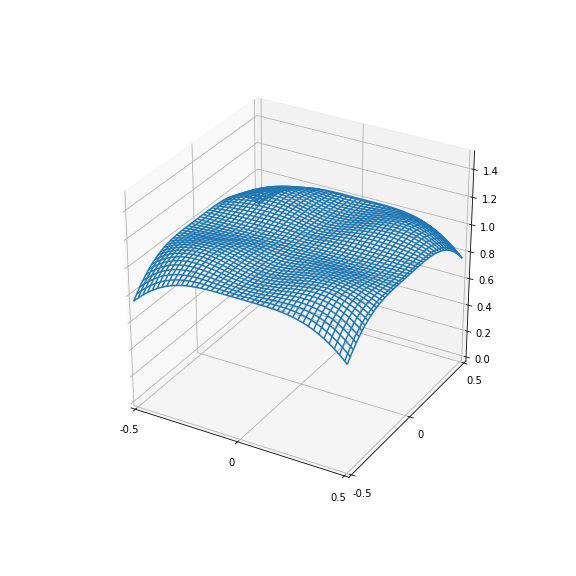
\includegraphics[width=0.8\linewidth]{3dcont.png}}
\caption{$\alpha = 0.00001\,,\gamma = 0.1$}
\end{figure}
\end{column}
\begin{column}{0.5\textwidth}
$$v(x,y) = e^{ikx}e^{ily}, k \neq 0, l \neq 0$$
$$g_1 = v_x =ixe^{ikx}e^{ily}$$
$$ g_2 = v_y = ile^{ikx}e^{ily}$$
\end{column}

\end{columns}
\begin{block}{Частотная характеристика при точных значением производных}
$$
H_{kl} = \frac{1}{u_{kl}} = \frac{(\frac{1}{k^2} + \frac{1}{l^2})\lambda_k\lambda_l}{\mu_l \lambda_k + \mu_k \lambda_l + \alpha \mu_k \mu_l + \gamma \lambda_k \lambda_l}
$$
\end{block}
\end{frame}


\begin{frame}
\frametitle{Частотные характеристики}
\framesubtitle{Случай точных значений производных}
\begin{columns}
\begin{column}{0.4\linewidth}
\begin{figure}[H]
\center{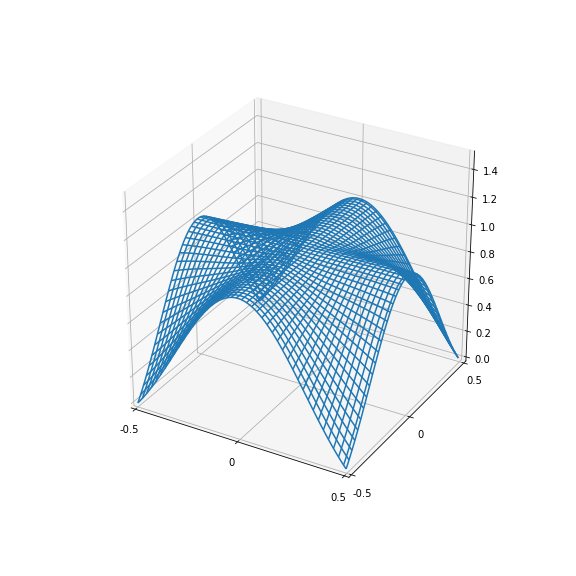
\includegraphics[width=0.9\linewidth]{3dpiece.png}}
\caption{$\alpha = 0.00001\,,\gamma = 0.1$}
\end{figure}
\end{column}
\begin{column}{0.5\textwidth}
$$(g_1, \phi_x) = \frac{4}{\omega_l h^2}  \sin^2\frac{\omega_k}{2}  \sin\,\omega_l e^{ikx_n}e^{ily_m}$$
$$(g_2, \phi_y) = \frac{4}{\omega_k h^2}  \sin^2\frac{\omega_l}{2}  \sin\,\omega_k e^{ikx_n} e^{ily_m}$$
\end{column}

\end{columns}
\begin{block}{Частотная характеристика в случае восстановления по средним локальным апертурам значений наклонов}
$$
H_{kl} = \frac{1}{u_{kl}} = \frac{\frac{\lambda_k \sin(lh_2)}{lh_1} + \frac{\lambda_l \sin(kh_1)}{kh_1}}{\mu_l \lambda_k + \mu_k \lambda_l + \alpha \mu_k \mu_l + \gamma \lambda_k \lambda_l}
$$
\end{block}
\end{frame}


\begin{frame}
\frametitle{Восстановление полинома Цернике $Z_2^{-2} = \rho^2 \sin(2\phi)$}
Точные значения производных:
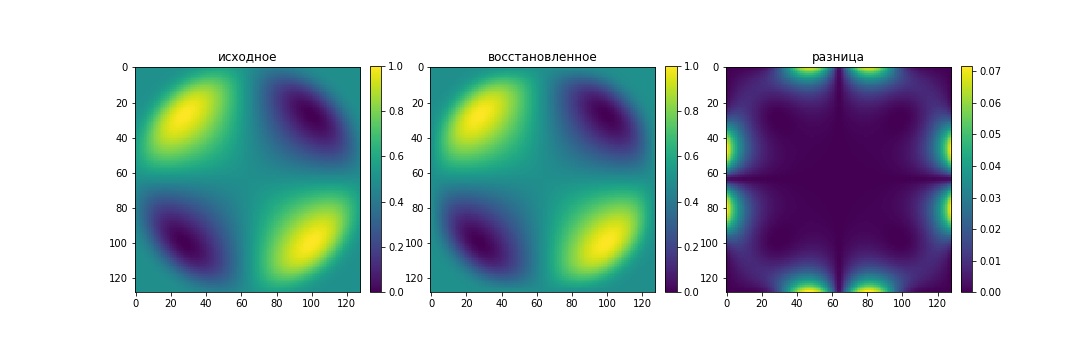
\includegraphics[width=1\linewidth]{z_2^-2.png}
\\
Случай восстановления по средним локальным апертурам значений наклонов:
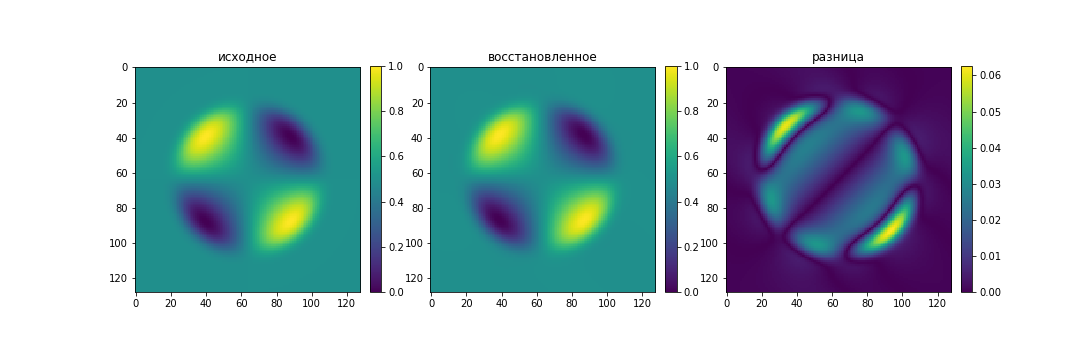
\includegraphics[width=1\linewidth]{z_2^-2_v2.png}


\end{frame}
\begin{frame}{Положения, выносимые на защиту}
\begin{enumerate}
\item Реализованы вейвлет и вариационный методы восстановления волнового фронта
\item Получена частотная характеристика вариационного метода для случая восстановления по средним локальным апертурам значений наклонов
\item Проведены вычислительные эксперименты, подтверждающие работоспособность методов
\item Удалось установить, что вейвлет метод идеален для случая первых разностных производных, но имеет существенную погрешность в остальных случаях, а вариационный метод имеет стабильные результаты для различных способов задания наклонов волнового фронта
\end{enumerate}
\end{frame}

\end{document}






